\section{Фальсификационные обязательства}
\label{sec:falsification}

Эта секция вынесена как отдельный структурный уровень, а не как параграф в Обсуждении, по причине, которую мы формулируем открыто. \DEIC{} претендует на масштаб, который в академической психологии традиционно вызывает скепсис --- не потому, что масштаб сам по себе подозрителен, а потому, что широкие рамки исторически редко говорили, \emph{при каком наблюдении они признают себя ошибочными}. Мы эту границу проводим сами, заранее и на видном месте. Ниже --- список предсказаний, каждое из которых сформулировано вместе со своим фальсификатором: наблюдением, при котором это предсказание следует считать опровергнутым. Опровержение каждого отдельно означает локальное обновление рамки; опровержение определённых комбинаций, указанных в §\ref{subsec:collapse_thresholds}, означает, что \DEIC{} как каркас подлежит структурному пересмотру или отзыву.

Формально, это не обещание быть правыми. Это обязательство признавать, когда мы неправы, и обязательство --- в каких именно местах и на каких именно данных проверка будет проведена.

\subsection{Ориентация в таблице обязательств}
\label{subsec:falsification_guide}

Каждое обязательство ниже имеет четыре компонента: \textbf{(1)}~утверждение (что \DEIC{} предсказывает или постулирует), \textbf{(2)}~фальсификатор (какое наблюдение делает утверждение ложным), \textbf{(3)}~требования к тесту (какой дизайн, какой размер выборки, какая инструментальная конфигурация необходимы для того, чтобы тест имел силу), \textbf{(4)}~последствие опровержения (что именно в рамке подлежит пересмотру, а не просто ослабляется). Обязательства сгруппированы по пяти тирам: измерительные (тир~А), причинно-путевые (тир~B), топологические (тир~C), архитектурные (тир~D) и программные (тир~E).

\begin{figure}[htbp]
\centering
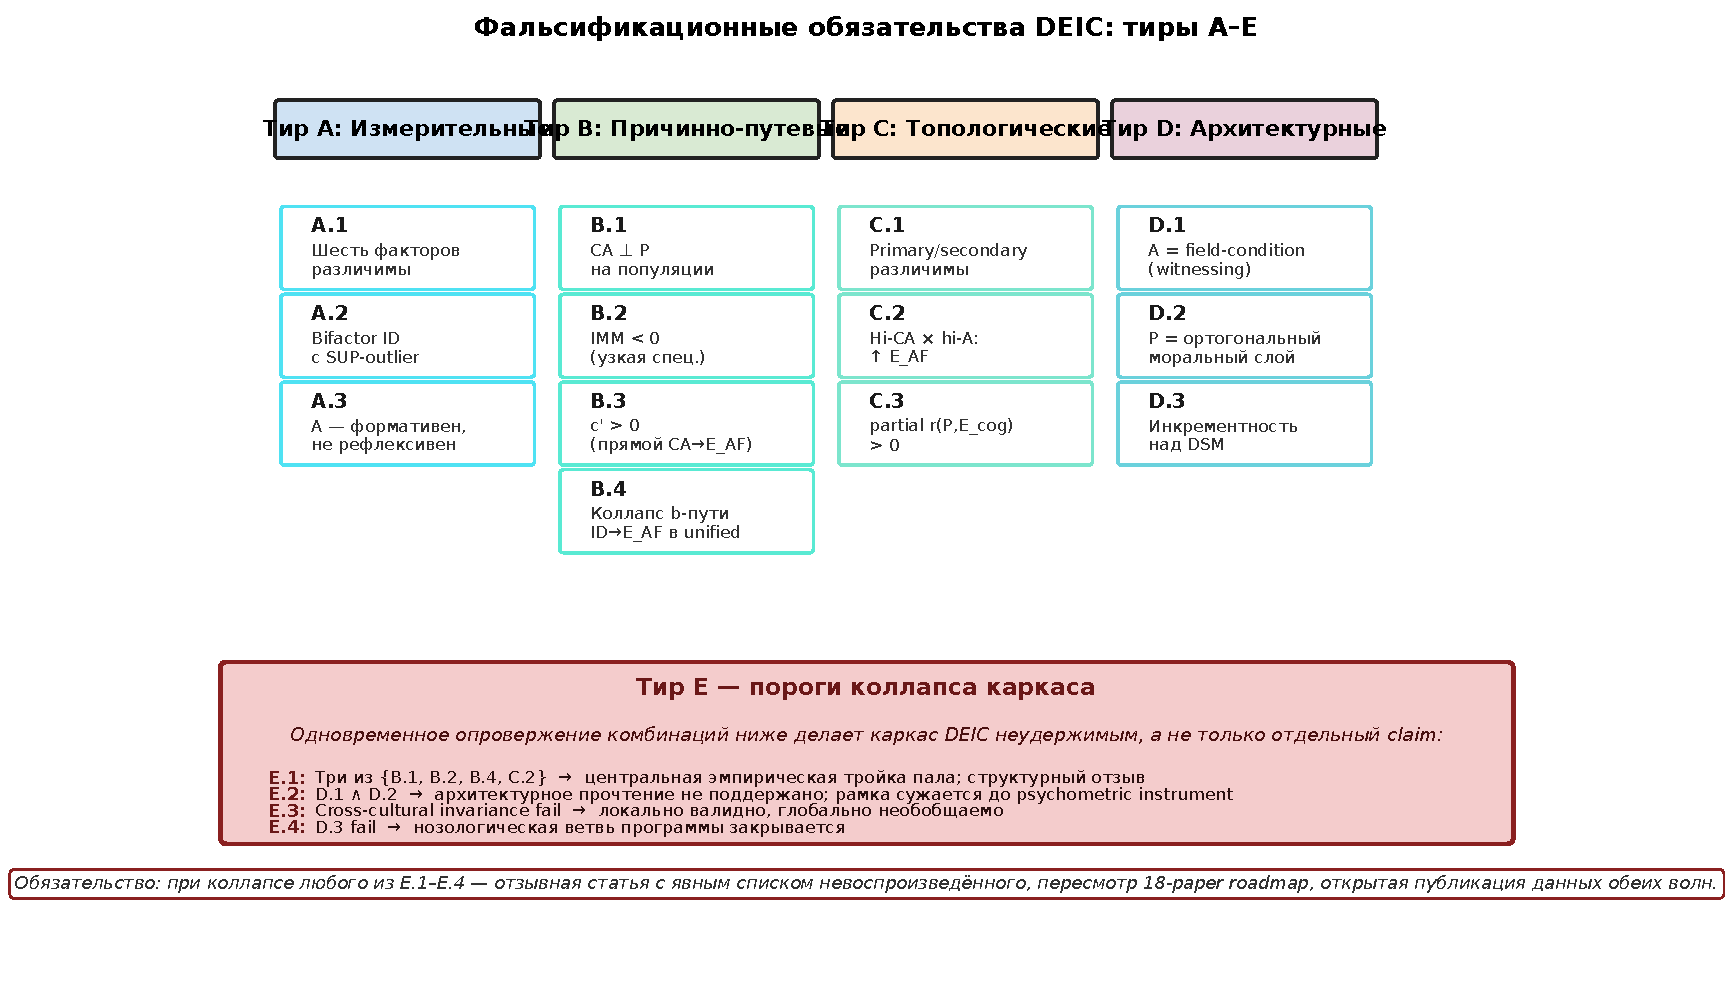
\includegraphics[width=0.95\linewidth]{figures/fig10_falsification_map.pdf}
\caption[Карта фальсификационных обязательств]{Карта фальсификационных обязательств \DEIC{}. Четыре тира локальных тестов (А --- измерение; B --- причинные пути; C --- топология; D --- архитектура) формируют верхний ряд, каждый со своими обязательствами. Нижняя красная полоса --- тир~E: пороги программного коллапса, при достижении которых каркас подлежит структурному пересмотру, а не локальному обновлению.}
\label{fig:falsification_map}
\end{figure}

Формулировки умышленно бинарны. Наука не работает в бинарных режимах --- но обязательства работают: либо мы готовы признать результат опровержением, либо мы его заранее выводим за рамки теста, и тогда это не обязательство.

\subsection{Тир А: измерительные обязательства}
\label{subsec:falsification_tier_a}

\paragraph{A.1 --- Шесть факторов различимы.}
\emph{Утверждение.} Шестифакторная oblique-CFA (ID, CA, P, M, \EAF{}, \Ecog{}) устойчиво воспроизводится на pre-registered айтемах, разведённых по дизайну.
\emph{Фальсификатор.} В волне~2 с айтемами, разведёнными по дизайну ($N \geq 1000$), либо \EAF{} и \Ecog{} сливаются в единый empathy-фактор (CFI модели с объединённой E не хуже чем с разделённой на $\Delta$CFI $\leq 0.01$), либо ID и CA неразличимы как отдельные латенты ($r_{\mathrm{lat}} > 0.90$), либо P и M неразличимы при условии инструментальной независимости.
\emph{Требования к тесту.} Pre-registered дизайн; айтемы для \EAF{} и \Ecog{} написаны по разным content-специфическим конструктам, не делят общие слова. $N \geq 1000$ для устойчивой CFA на 6 факторах.
\emph{Последствие опровержения.} Многомерная архитектура эмпатии в текущем виде не поддержана; \DEIC{} сужается до факторной структуры, которую данные держат (возможно, четырёх- или пятифакторной).

\paragraph{A.2 --- Bifactor-структура ID с SUP-как-отдельным.}
\emph{Утверждение.} ID-umbrella лучше описывается bifactor-моделью (общий ID$_{\mathrm{g}}$ плюс пять uncorrelated specific-факторов), чем однофакторной, при $\Delta\chi^2$-тесте с $p < 0.001$. Per-subscale ECV для SUP остаётся ниже $0.45$, для FLA выше $0.70$.
\emph{Фальсификатор.} В волне~2 bifactor-модель не превосходит однофакторную по $\Delta\chi^2$ при $p < 0.01$, ИЛИ ECV для SUP $> 0.55$ (SUP одинаково хорошо поглощается общим ID), ИЛИ ECV для FLA $< 0.45$ (FLA перестаёт быть чистым индикатором общего ID).
\emph{Требования к тесту.} $N \geq 1200$ с айтемами для SUP, восстановленными как самостоятельный латент по дизайну волны~2.
\emph{Последствие опровержения.} Гипотеза «пассивное блокирование --- единая архитектура с поверхностными вариациями» подлежит пересмотру; возможна пере-сегментация ID на два независимых латента.

\paragraph{A.3 --- A формативен, не рефлексивен.}
\emph{Утверждение.} A в текущем инструменте работает как формативный композит. Выделенная A-шкала, написанная по дизайну на чистый witnessing (наблюдение-наблюдения без trauma-hypervigilance), даст рефлексивный единофакторный CFI $\geq 0.93$ и воспроизведёт отрицательный \IMM{} в узкой спецификации.
\emph{Фальсификатор.} Dedicated witnessing-A-шкала даёт CFI единичного латента $\geq 0.95$ \emph{и} \IMM{}, воспроизводящий знак и направление композитного $-0.00197$ (CI не включает ноль) --- тогда A рефлексивен, и наш аргумент о его формативности ложен. Либо, наоборот, witnessing-шкала даёт CFI $< 0.85$ и \IMM{} незначим --- тогда ни одна из операционализаций A не поддерживает гипотезу witnessing-модерации.
\emph{Требования к тесту.} Item-level разведение witnessing (Josipovic/Dunne/Grabovac-anchor items) и hypervigilance (trauma-focused items); $N \geq 800$; вложенная conditional-process SEM.
\emph{Последствие опровержения (обе ветви).} Либо A реинтерпретируется как рефлексивный конструкт (упрощение), либо гипотеза witnessing-модерации не поддержана (пересмотр центрального claim о роли внимания).

\subsection{Тир B: причинно-путевые обязательства}
\label{subsec:falsification_tier_b}

\paragraph{B.1 --- CA$\perp$P на популяционном уровне.}
\emph{Утверждение.} В параллельной медиации CA$\to$\{ID, P, M\}$\to$\EAF{} путь CA$\to$P остаётся близким к нулю ($|\beta| < 0.10$) в репликации с выборкой, сопоставимой по ширине CA-спектра.
\emph{Фальсификатор.} CA$\to$P $\beta > 0.20$ при $p < 0.01$ в репликационной выборке $N \geq 1000$, с CA-инструментом и P-инструментом сопоставимого содержания.
\emph{Требования к тесту.} Репликация на независимой выборке; CA-инструмент покрывает тот же спектр (раннее реляционное пренебрежение, насилие, эмоциональная депривация); P-инструмент сохраняет долю моральной и архитектурной подписи.
\emph{Последствие опровержения.} Архитектурная ортогональность P и CA не поддержана; первичная/вторичная психопатия становится континуумом, а не топологически отдельными клетками. Следствие для клиники: психопатический паттерн снова интерпретируется как (ко)-исход детской травмы, а не как отдельная архитектура.

\paragraph{B.2 --- \IMM{} в узкой спецификации отрицателен.}
\emph{Утверждение.} В conditional process SEM без P в $b$-уравнении \IMM{} канала CA$\to$ID$\to$\EAF{} отрицателен, 95\% CI не включает ноль.
\emph{Фальсификатор.} $P(\mathrm{IMM} < 0) < 0.90$ под любым из трёх референсных байесовских приоров на репликационной выборке, ИЛИ CI frequentist-оценки пересекает ноль при $N \geq 1000$ и сопоставимой структуре A-композита.
\emph{Требования к тесту.} A-композит с сопоставимой весовой структурой; репликация проводит параллельный байесовский и частотный анализ.
\emph{Последствие опровержения.} Центральный результат статьи (двухстадийная A-модерация CA$\to$ID$\to$\EAF) не поддержан; A как модератор канала в узкой спецификации пересматривается.

\paragraph{B.3 --- $c'$ (прямой путь CA$\to$\EAF{}) положительный.}
\emph{Утверждение.} После partialling ID, P, M и A прямой путь CA$\to$\EAF{} остаётся положительным ($+0.15$--$+0.25$) --- «сырая» детская травма не убивает эмпатию сама; её убивает защитный каскад.
\emph{Фальсификатор.} $c' < -0.10$ с $p < 0.01$ в репликации, после корректного partialling.
\emph{Требования к тесту.} Репликация с сохранением структуры медиаторов; контроль на response bias (Lie как ковариата \EAF).
\emph{Последствие опровержения.} Ключевой тезис введения («травма не приговор; её транслирует защита») лишается опоры; DEIC-рамка переходит к более стандартному «травма $\to$ эмоциональное повреждение» нарративу.

\paragraph{B.4 --- В unified SEM $b$-путь ID$\to$\EAF{} коллапсирует.}
\emph{Утверждение.} При одновременной оценке всех путей в unified SEM коэффициент ID$\to$\EAF{} падает до статистической незначимости ($|\beta| < 0.10$, $p > 0.05$), а P$\to$\EAF{} доминирует.
\emph{Фальсификатор.} В репликации $b$-путь ID$\to$\EAF{} остаётся $\beta < -0.20$ при $p < 0.001$ даже при включении P в то же уравнение.
\emph{Требования к тесту.} Репликация unified SEM с той же структурой латентов.
\emph{Последствие опровержения.} Разведение «архитектурного» и «нарративного» слоёв в модели \EAF{} не поддержано; P и ID оказываются скорее аддитивными, чем иерархическими, медиаторами, и теоретическое разделение ортогональных каналов требует пересмотра.

\subsection{Тир C: топологические обязательства}
\label{subsec:falsification_tier_c}

\paragraph{C.1 --- Первичная и вторичная психопатия топологически различимы.}
\emph{Утверждение.} В подвыборке hi-P ($N \geq 200$) наблюдается бимодальность на оси ID (или, в многомерной версии, две различимые кластера в плоскости ID$\times$CA), соответствующая Karpman-различению: первичная клетка (ID $\approx 0$, CA $\approx 0$) и вторичная (ID $> +0.5$, CA $> +0.5$).
\emph{Фальсификатор.} В hi-P подвыборке $N \geq 200$ Hartigan dip-тест не даёт свидетельства бимодальности ($p > 0.1$), ИЛИ Gaussian mixture на (ID, CA, A) даёт лучший BIC для $k=1$, чем для $k=2$.
\emph{Требования к тесту.} Репликация на независимой выборке; желательно клинически обогащённой hi-P подгруппой.
\emph{Последствие опровержения.} Karpman-различение на DEIC-координатах не поддержано; топологический $2\times2$ схлопывается до continuum psychopathy, как в большей части современной литературы. Следствие для клиники: разные интервенции для «первичного» и «вторичного» типа лишаются опоры.

\paragraph{C.2 --- Интегрированный выживший имеет повышенную \EAF{}.}
\emph{Утверждение.} Клетка hi-CA $\times$ hi-A ($\geq$ медианы по каждой оси; ожидаемая доля $\sim 15$--$18\%$ выборки) имеет \EAF{}, превышающий медиану общей выборки и превышающий клетку hi-CA $\times$ lo-A хотя бы на $0.4\sigma$.
\emph{Фальсификатор.} $\mathrm{mean}\ \mathrm{E_{AF}}$ в клетке hi-CA $\times$ hi-A ниже или равен медиане общей выборки ($\Delta \leq 0$), ИЛИ разница с hi-CA $\times$ lo-A $< 0.2\sigma$ в репликации $N \geq 1000$.
\emph{Требования к тесту.} Репликация с аналогичной операционализацией A (композит или эквивалентная witnessing-шкала); выборка включает достаточную hi-CA представительность ($\geq 25\%$).
\emph{Последствие опровержения.} Центральный публично-значимый claim о том, что witnessing-работа компенсирует CA-эффект на аффективную эмпатию, не поддержан; «травма не приговор» как эмпирическое утверждение отзывается, остаётся как клинический горизонт без статистической опоры.

\paragraph{C.3 --- Partial $r$(P, \Ecog) положителен.}
\emph{Утверждение.} После partialling ID и CA частная корреляция P и \Ecog{} остаётся положительной ($> +0.15$). Это объясняется hyper-instrumentation: P-паттерн использует распознавание чужих состояний избирательно, не являясь дефицитным на cognitive-E оси.
\emph{Фальсификатор.} Partial $r$(P, \Ecog{} \textbar{} ID, CA) $\leq 0$ в репликации $N \geq 1000$ со сравнимым разведением \EAF{}/\Ecog{}.
\emph{Требования к тесту.} \Ecog{}-шкала написана на perspective-taking и understanding-of-others, а не на empathic concern; P-шкала сохраняет моральную и архитектурную долю; айтемы не делят слова.
\emph{Последствие опровержения.} Hyper-instrumentation-гипотеза Blair/Baron-Cohen в наших данных не воспроизводится; «классическое» описание психопатии как дефицитной в обеих формах эмпатии оказывается точнее. Рамка «архитектура, не дефицит» на оси E ослабляется.

\subsection{Тир D: архитектурные обязательства}
\label{subsec:falsification_tier_d}

\paragraph{D.1 --- A как field-condition, не как содержание поля.}
\emph{Утверждение.} Dedicated witnessing-A-шкала, разведённая по дизайну с trauma-hypervigilance, даёт тот же знак и направление модерации канала CA$\to$ID$\to$\EAF, что и текущий композит A. Если же конструируется чистая hypervigilance-шкала (только внимание-к-внутреннему без witnessing), она модерирует канал в противоположном направлении либо не модерирует его вовсе.
\emph{Фальсификатор.} Обе шкалы (witnessing-only и hypervigilance-only) модерируют канал в одном и том же направлении в репликации, ИЛИ witnessing-шкала не модерирует вовсе.
\emph{Требования к тесту.} Два параллельных item-set, контентно-валидизированных экспертами в созерцательной традиции и в trauma-психологии; одна и та же структура SEM для обеих.
\emph{Последствие опровержения.} Онтологическое различение witnessing vs content at the attention-axis не поддержано; A возвращается в общий ряд компонентов dispositional attention, связь с не-двойственной созерцательной традицией лишается эмпирической опоры (остаётся теоретической).

\paragraph{D.2 --- P как ортогональный моральный слой.}
\emph{Утверждение.} Cognitive-morally phrased P-айтемы («я считаю, что в моём случае такое поведение допустимо») дают $\beta$ на \EAF{} и партиальные корреляции с architectural-P-айтемами такие, что P-композит сохраняет $\approx$ половину своей дисперсии как моральную компоненту и $\approx$ половину как архитектурную. P-moral в одиночку остаётся ортогональным CA ($|\beta| < 0.10$).
\emph{Фальсификатор.} После разведения P на P-moral и P-arch в волне~2 обе компоненты оказываются либо $r_{\mathrm{lat}} > 0.85$ (неразличимы), либо P-moral коррелирует с CA на $\beta > +0.25$.
\emph{Требования к тесту.} Pre-registered item-split; $N \geq 1000$; явные cognitive-moral vs architectural формулировки.
\emph{Последствие опровержения.} Моральный слой P не различим от архитектурного; интерпретация психопатии как «условное сцепление плюс нарратив разрешения» становится внутренне неоперабельной, сводится к одной архитектурной компоненте. Этическая рамка «архитектура морально нейтральна; нарратив оценим» лишается эмпирической отсечки.

\paragraph{D.3 --- Инкрементная валидность DEIC-профиля над DSM-меткой.}
\emph{Утверждение.} В retrospective re-analysis клинических датасетов с treatment response как outcome DEIC-профиль на baseline объясняет по крайней мере 5\% дополнительной дисперсии ответа после partialling DSM-метки.
\emph{Фальсификатор.} В ретроспективе на клинических данных $N \geq 2000$ с измеренным DEIC-профилем инкрементная $R^2$ над DSM $< 0.05$.
\emph{Требования к тесту.} Одна или несколько клинических выборок с параллельным DEIC-измерением и DSM-диагностикой; outcome: treatment response на стандартизованной метрике (HAMD, PHQ, BDI, etc.).
\emph{Последствие опровержения.} Нозологическая претензия DEIC как trans-diagnostic stratifier не поддержана; рамка сужается до описательно-теоретической роли без претензии на клиническую пере-организацию.

\paragraph{D.4 --- DI как архитектурный маркер, а не индикатор social desirability.}
\emph{Утверждение.} Величина декларативно-поведенческого разрыва $DI_{overall}$ трекает защитный латент ID ($r \geq +0.30$) и witnessing-латент A ($r \leq -0.30$) и не трекает клинический диагноз ($|r| < 0.15$) в wave-2 на независимой выборке. Prosocial-выровненная версия $DI_{aligned}$ остаётся структурно различимой с $piz$ ($|r| < 0.50$ с обратным знаком от ожидаемого, если бы DI был самопрезентационным индикатором).
\emph{Фальсификатор.} В wave-2 ($N \geq 800$) либо $|r(DI_{overall}, \text{ID})| < 0.30$, либо $|r(DI_{overall}, \text{dx\_any})| > 0.20$, либо $r(\text{piz}, DI_{aligned}) > +0.30$ (превращает DI в sub-компонент $piz$ без самостоятельной диспозиции).
\emph{Требования к тесту.} Wave-2 inventory с сохранённым принципом парных декларативных/поведенческих формулировок на всех шкалах ID-периметра; переизмерение dx и piz на той же выборке; re-fit 6-factor oblique CFA с латентными scores.
\emph{Последствие опровержения.} DI как самостоятельная архитектурная метрика не поддержан: либо разрыв не трекает архитектуру, либо он трекает клинический профиль (что переводит DI в диагностическую, а не архитектурную категорию), либо он полностью объясняется $piz$ (чистый SD-артефакт). В любом из этих случаев параграф §\ref{subsec:di_asymmetry} и интерпретация DI в §\ref{subsec:di_results} требуют ретракции; \texttt{extended\_metrics.DI} в инструменте из архитектурного маркера становится либо клиническим, либо дубликатом $piz$, и его место в wave-2 дэшборде пересматривается.

\subsection{Тир E: программные пороги коллапса}
\label{subsec:collapse_thresholds}

До сих пор каждое обязательство описано как локальный тест с локальным последствием. Однако \DEIC{} --- не набор независимых гипотез, а архитектура с взаимозависимыми узлами. Опровержение определённых комбинаций означает, что каркас в целом не держит, а не только что одна ветка устарела. Мы формулируем эти комбинации явно.

\paragraph{E.1 --- Коллапс центральной эмпирической тройки.}
Если одновременно опровергнуты три из четырёх центральных обязательств --- B.1 (CA$\perp$P), B.2 (\IMM{} отрицателен), B.4 (коллапс $b$-пути в unified), C.2 (интегрированный выживший с повышенной \EAF{}) --- три из эмпирических столпов, на которых построен центральный аргумент статьи, не воспроизводятся. В этом случае \DEIC{} как эмпирическая рамка подлежит \emph{структурному пересмотру, а не обновлению}: версия~2 инструмента и сопутствующая теоретическая рамка должны быть отозваны и заменены сужённой рабочей гипотезой с явным указанием тех фрагментов, которые в этой точке ещё поддерживаются.

\paragraph{E.2 --- Коллапс архитектурного прочтения.}
Если опровергнуты одновременно D.1 (witnessing-модерация) и D.2 (различимость P-moral и P-arch), теоретическая рамка «психопатия как условное сцепление плюс моральный нарратив; внимание как field-condition» не поддержана. \DEIC{} в этом случае \emph{сужается до эмпирической координатной системы} без архитектурных и онтологических тезисов: пригодна как psychometric instrument, но не как рамка, претендующая на диалог с созерцательной традицией и с моральной философией.

\paragraph{E.3 --- Коллапс обобщаемости.}
Если cross-cultural валидация на не-русскоязычных выборках (EN, ES, CH, AR) показывает, что шестифакторная CFA не воспроизводит scalar invariance, а центральные B.2 и C.2 воспроизводятся лишь в \emph{части} культурных контекстов, \DEIC{} остаётся \emph{локально валидным, глобально необобщаемым} инструментом. Это не коллапс рамки как таковой, но отзыв претензии на то, что описанная архитектура --- универсальный устройство психики, а не артефакт русскоязычной/поздне-советской культурной формации. Прикладные статьи программы (политическая коммуникация, эволюционная психология) в этом случае ограничиваются соответствующим культурным диапазоном.

\paragraph{E.4 --- Коллапс нозологической претензии.}
Если опровергнут D.3 (инкрементная валидность над DSM), нозологическая ветвь программы (статья о DEIC-профиле как trans-diagnostic stratifier, §\ref{sec:future}) закрывается до появления новых оснований. Рамка остаётся описательно-научной, но не претендует на пере-организацию клинических категорий.

\paragraph{Что означает «каркас подлежит пересмотру».}
Нами признано: публичный отзыв или структурный отзыв не тождественны тихому molchaniyu. В случае коллапса любого из уровней E.1--E.4 мы обязуемся \textbf{(i)}~опубликовать отзывную статью с явным списком того, что не воспроизводится, и с явной переформулировкой того, что остаётся; \textbf{(ii)}~пересмотреть программу публикаций \S18-paper roadmap --- некоторые из планируемых статей потеряют основания и будут сняты; \textbf{(iii)}~опубликовать данные обеих волн открыто, чтобы другие группы могли проводить независимые ре-анализы. Это обязательство имеет ту же форму, что и обязательства открытой методологической культуры после кризиса репликации в социальной психологии 2010-х годов: не «если мы ошибёмся, мы перепишем историю», а «если мы ошибёмся, мы признаем и отдадим данные».

\subsection{Что означает этот раздел для чтения статьи}
\label{subsec:falsification_closing}

Мы формулируем два следствия для читателя.

Первое. Никакое утверждение этой статьи не следует читать как «закрытый» или «доказанный» факт. Каждое --- гипотеза со своей границей фальсификации, сформулированной здесь. В тексте статьи --- в Результатах, в Обсуждении --- эти утверждения формулируются в findings-регистре («данные показывают», «модель даёт»), как этого требует психометрическая отчётность. Но научный статус каждого из них определяется не этим регистром, а наличием сформулированного фальсификатора в этой секции.

Второе. Мы не рассматриваем фальсификацию как угрозу программе. Опровержение локального предсказания (любого из A.1--D.3) --- это нормальный ход эмпирического исследования и основание для обновления. Опровержение комбинации (E.1--E.4) --- это нормальный ход научной самокоррекции, и программа предусматривает такой исход как возможный. Единственный неприемлемый для нас исход --- не опровержение, а ускользание: если утверждения сформулированы так, что их нельзя ни подтвердить, ни опровергнуть, то работа выходит за пределы науки независимо от своей технической сложности. Фальсификационная секция существует именно для того, чтобы такого ускользания не было. Это --- вклад, который мы считаем независимым от того, окажется ли сама рамка валидной.

В §\ref{sec:future} сформулированы конкретные дизайны, которые будут проводить каждый из тестов. В открытой документации программы (\texttt{PROGRAM\_STRUCTURE.md}) указаны запланированные статьи и их привязка к тирам A--E этой секции.
